\chapter{Conclusions}
\label{cha:conclusions}

\section{Summary of results}

The main findings of this thesis are summarised as follows: 
%\begin{enumerate}

\bigskip\noindent\textbf{Application of moment diagnostics.} It has been
demonstrated that vortex moment diagnotsics can be successfully applied to the
geopotential height field, giving similar results as when applied to
conservative fields such as PV. This therefore provides a semi-Lagrangian (or
vortex-centric) method which can be readily used to describe the geometry of the
stratospheric polar vortex in climate model simulations.

It has been further shown that a simple threshold-based method can be applied to
the vortex moment diagnostics in order to indentify split and displaced vortex
events. The events identified in this way coincide to a large extent with events
defined by other methods, and capture equally extreme vortex states.

\bigskip\noindent\textbf{The stratospheric polar vortex in climate models.} The
first multi-model comparison of stratospheric polar vortex geometry and split an
displaced vortex events has been carried out using the stratosphere-resolving
CMIP5 models. A wide range of biases have been identified in the geometry of the
stratospheric polar vortex among models. Some models have a vortex which is on
average too equatorward, others too poleward, while the majority of models have
a vortex which is too circularly symmetric. Models also vary widely in their
frequency of split and displaced vortex events. However, the nature of these
events is largely in agreement with observations, in particular the fact that
split vortex events appear more barotropic and displaced vortex events
baroclinic. The consistency of this difference in baroclinicity among models
lends weight to the idea that split vortex events are caused by a resonant
excitation of the barotropic mode, as suggested by
\citet{Esler2005}. Significantly, the frequency of split and displaced vortex
events has been demonstated to be highly correlated respectively with the aspect
ratio and centroid latitude of the average vortex state. It therefore follows
that an improvement in the mean state of the vortex is likely to lead to a more
accurate representation of these extremes.

\bigskip\noindent\textbf{Stratosphere-troposphere coupling in climate models and
  observations.}  In reanalysis data, using the geopotential height-based vortex
moments method, a stronger tropospheric NAM signal is seen following split
vortex events than displaced vortex vortex events. This is in agreement with the
results of \citet{Mitchell2013}. However, a bootstrap significance test of the
surface NAM over the month following these events cannot exclude the possibility
that this observed difference is due to chance.

In the CMIP5 models, the tropospheric NAM signal following both split and
displaced vortex events is weak on average. There is no consistent difference
between the two apart from close to the onset of events when there is a negative
anomaly for split vortex events which extends barotropically through the depth
of the atmosphere. However, looking at two-dimensional tropospheric anomalies in
mean sea-level pressure following split and displaced vortex events shows some
consistent features. A negative NAO-like signal is seen which is of similar
magnitude following both types of event. The Pacific response is much less
robust, with some models simulating negative pressure anomalies, and others
positive. The discrepancy between the Atantic and Pacific responses suggests
that the annular mode may not be a good metric for stratosphere-troposphere
coupling in the NH.

Almost all models show more negative sea-level pressure anomalies over Siberia
following displaced vortex events than split vortex events. Overall, the
differences in the surface signals following the two types of events are
approximately co-located with the difference in lower-stratospheric geopotential
height, which in turn follow stratospheric PV anomalies. A similar pattern is
also seen in tropopause height in reanalysis data. This suggests the mechanism
behind the different surface responses to split and displaced vortex events is
one local to lower stratospheric PV anomalies, as proposed by
\citet{Ambaum2002}. However, it should be stressed that the similarities in the
NAO response suggest that other mechanisms more sensitive to zonal-mean
anomalies, such as baroclinic instability or planetary wave reflection, also
play a role.

\bigskip\noindent\textbf{Predictability of the polar stratosphere.} Using
hindcast simulations produced by a stratosphere-resolving seasonal forecast
system, no skill has been found in the prediction of NH SSWs or split or
displaced vortex events at lead times beyond one month. This suggests that the
skillful seasonal prediction of the winter NAO in the same system
\citep{Scaife2013} is not highly influenced by the stratosphere. It may,
however, be attributable to other model improvements such as increased
atmospheric and oceanic horizontal resolution.

On the other hand, skillful prediction of the SH stratospheric polar vortex
during the austral spring at seasonal lead times has been found. This skill is
greater than a persistence forecast; indeed, a strong late-summer polar vortex
is related to a weak spring vortex, indicating the importance of
preconditioning. Using the observed relationship between the strength of the
stratospheric polar vortex and polar ozone, it was possible to produce skillful
forecasts of interannual variations in polar stratospheric ozone depletion. This
prediction is at longer lead times than previous forecasts. Furthermore, because
interannual variability is significant when compared to the long-term ozone
depletion trend, such forecasts may be of some interest for populations in the
SH.

A further feature of the hindcast simulations is that the year 2002, in which
the only observed SH SSW occurred, is also the most extreme of the hindcasts
with almost all ensemble members simulating negative stratospheric wind
anomalies. It also has one of the two out of 210 ensemble members which simulate
SH SSW-like events (although these are displaced vortex events, rather than the
split that occurred). This suggests that an increased likelihood of the 2002
event may have been detectable almost two months in advance.

\bigskip\noindent\textbf{Stratospheric influence on tropospheric
  predictability.} The same seasonal forecast stystem produces forecasts of the
austral spring mean surface SAM at one month lead times. It also accurately
simulates the surface temperature pattern associated with the SAM, such that the
SAM forecast skill leads directly to skilful surface temperature forecasts over
much of Antarctica, New Zealand, and eastern Australia. Interestingly, these
forecasts were found to be more skilful during October--November (2 month lead
time), than September (1 month lead time). The same pattern is replicated in a
statistical hindcast which takes as its only input the polar-cap mean
geopotential height at 10~hPa on 1st August. The pattern cannot, however, be
replicated by a statistical forecast based on the ENSO index. This suggests,
therefore, that the tropospheric skill during October-November is largely
attibutable to the influence of the predictable stratosphere during this
time. The October--November stratospheric SAM is, in turn, highly predictable due
to a strong negative correlation with the 1st August stratospheric SAM. The fact
that the stratospheric influence is greatest in October-November is also
backed-up by obervational evidence which shows the largest stratosphere-leading
correlations with the surface during this time. These results highlight the
importance of including a well-resolved stratosphere and accurate stratospheric
initial conditions in seasonal forecast systems. 

%\end{enumerate}

\section{Extensions of this work}

The work presented in this thesis has raised a number of questions, and
motivated future investigations. Some of these ideas are discussed below:

\bigskip\noindent\textbf{Decadal variability.} Looking by eye at the events
detected in Chapter \ref{cha:moments}, it appears that they cluster in time. For
instance, there are 10 events in the 1970s, but only 4 in the 1990s. Figure
\ref{fig:decadal} shows an attempt to analyse whether this decadal variability
is statistically significant. It shows (solid black line) the frequency of given
numbers of split/displaced vortex events within a 10-year moving window
(shifting by one year at a time) in the ERA data set. Also shown (dashed black
line) is the same calculation applied to randomly shuffled events. Error bars
are calculated from the distribution of frequencies of the randomly shuffled
events. It can be seen that the frequencies of 8/9 events and 3 events per
decade are sightly statistically significant from the random
variability, so it might be inferred that there is statistically significant
decadal variability. 

Figure \ref{fig:decadal} also shows the same calculation applied to a 2 ensemble
member 1860--2005 historical simulation of the HadGEM2-CC model (a total of 290
years). It can be seen in this case that the simulation is not distinct from
random variability. However, \citet{Schimanke2011} did find significant decadal
variability in a coupled ocean-atmosphere GCM, although their model simulated
only 2 events per decade. A future investigation could aim to resolve this issue
by studying decadal variability in a greater number of models (such as the CMIP5
ensemble). Longer simulations than those studied in Chapter \ref{cha:models}
would be required in order to achieve statistically signifiant results. It would
also be interesting to compare historical and control simulations in order to
determine if any decadal variability is externally driven or internally
generated.

\begin{figure}[t]
  \centering
  \noindent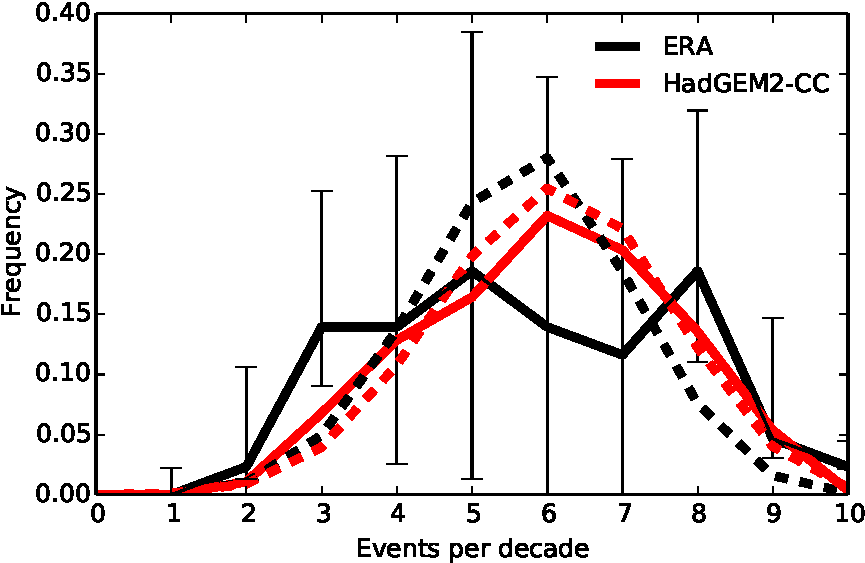
\includegraphics[width=0.6\textwidth,angle=0]{figures/chapter-conclusions/events_decadal.pdf}\\
  \caption[Decadal variability of SSWs]{(solid lines) Normalised frequency of
    the number of SSWs detected in a 10-year moving window. (dashed lines)
    Average of 10-year moving window frequency of SSWs whose timing is shuffled
    randomly 1000 times. Error bars depict the 2.5--97.5\%
    range of the randomly shuffled events.}\label{fig:decadal}
\end{figure}

\bigskip\noindent\textbf{Systematic variation of model resolution.} It was shown
in Figure \ref{fig:aspect_vert_res} that among CMIP5 models their appears to be
a relationship between the average aspect ratio of the stratospheric polar
vortex and vertical resolution, particularly in the
upper-troposphere/lower-stratosphere. Although this relationship is backed up by
the physical understanding of the influence fine-scale vertical structure on
planetary wave propagation in this region, it is not highly statistically
significant. Furthermore, the relationship does not hold when models of the same
family but different resolution are compared. These issues could be resolved by
performing a series of model integrations in which only the vertical resolution
is changed. The climatology of the stratospheric polar vortex would be studied
for each integration, and it could be determined if this relationship holds. If
it does, it could then be found at which point the vertical resolution is
sufficient for a relatively realistic average vortex state, which would be
valuable for modelling centres. Such a study need not be highly computationally
expensive since it involves studying the mean state (rather than extremes such
as SSWs), so relatively few years need to be simulated. 

\bigskip\noindent\textbf{??Time scale of stratosphere-troposphere coupling.} In
this thesis it has been demonstrated that split vortex events occur
barotropically, suggesting an excitation of the barotropic mode. The relative
roles of modes of variability can be further investigated though a decomposition
of temporal modes and then studying coherence between stratospheric and
tropospheric modes. This is traditionally carried out through a Fourier spectrum
analysis, however, the more modern technique of empirical mode decomposition
(EMD) \citep{Huang1998} may be more suited to this application. EMD has also
been used in atmospheric science by \citet{Coughlin2004}. The method decomposes
a given timeseries into a finite number of `modes', each of which have a
characteristic frequency. Unlike Fourier analysis, however, this frequency is
allowed to vary to some degree, so the modes need not be perfectly periodic. As
such, it is more applicable to time series of finite length and with a
pronounced seasonal variability, such as the NAM. I have performed a preliminary
analysis Figure \ref{fig:emd} shows an example of such analysis applied to NH
polar-cap average geopontential height. Further investigations can be carried
out to analyse the physical relevence of the modes and coherence between the
stratosphere and troposphere.

\begin{figure}[t]
  \centering
  \noindent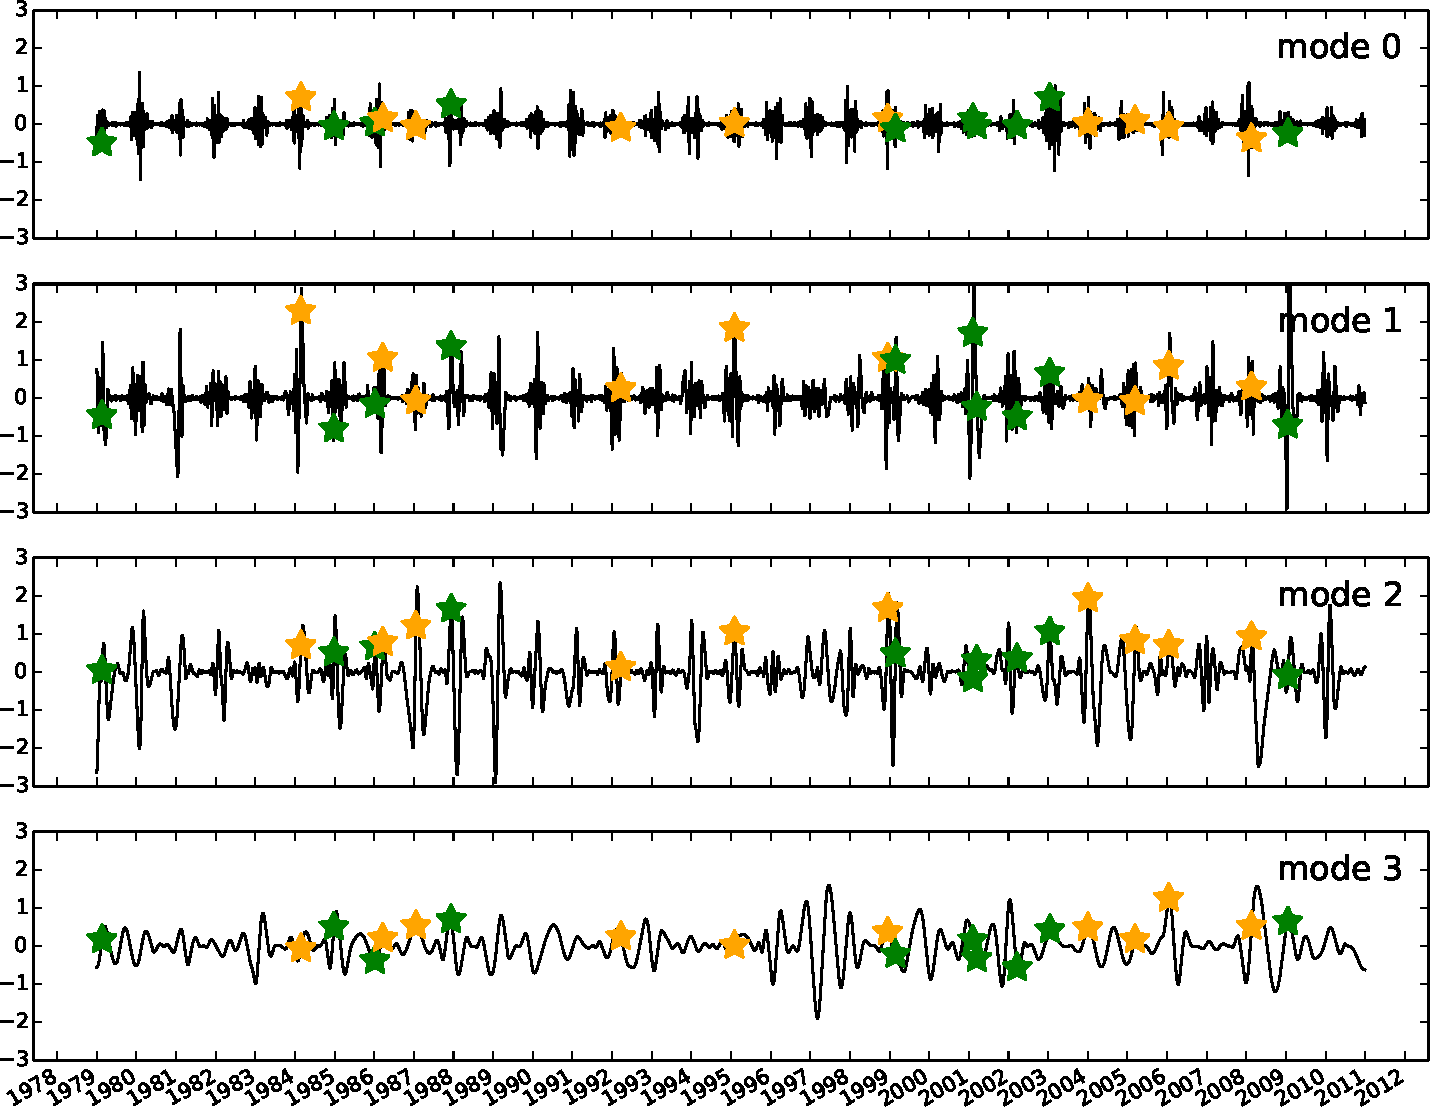
\includegraphics[width=\textwidth,angle=0]{figures/chapter-conclusions/EMD.pdf}\\
  \caption[EMD timeseries]{First four empirical modes of NH (60-90$^{\circ}$N)
    geopotential height in ERA-Interim data. Yellow and green stars represent
    displaced and split vortex events respectively.}\label{fig:emd}
\end{figure}


\bigskip\noindent\textbf{The 2002 Southern Hemisphere SSW.} The possibility of
an incresed likelihood of the 2002 SH SSW up to two months in advance was
suggested in Chapter \ref{cha:seas}. It is unclear, however, what factors
influence this predictability. It would therefore be interesting to carry out an
investigation in which possible influences are systematically changed. For
instance, the 2002 hindcasts could be re-run with an opposite phase of the QBO,
different tropical Pacific or Southern Ocean SSTs, or different polar
stratospheric initial conditions. The change in forecasts of the stratospheric
polar vortex could then be analysed, indicating which factors are most
important. It is likely that there would be some difficulty in imposing these
different initial conditions consistently. Furthermore, such an investigation is
likely to be quite computationally expensive as it is likely that many ensemble
members will be needed in order for a sufficient number of SSWs to be
simulated. 

\bigskip\noindent\textbf{Influence of interactive chemistry on seasonal forecast
  skill.} The seasonal forecast system analysed in Chapter \ref{cha:seas} did
not include interactive chemistry, with ozone concentrations set to a
climatology. It is therefore unable to capture the feedback between ozone
concentrations and the stratospheric circulation, or zonal asymmetries in
ozone. \citet{Waugh2009} have suggested that such asymmetries could have a
significant impact on tropospheric climate. This motivates an investigation as
to whether improved stratospheric or tropospheric forecasts may be achieved by
including interactive chemistry in a seasonal forecast system. Such a chemistry
scheme is likely to be expensive, so the investigation should determine which
reactions have the most impact on forecast skill.  



%%% Local Variables:
%%% mode: latex
%%% TeX-master: "thesis"
%%% End:
